%=========================================================================
% (c) Radim Loskot, 2014

\chapter{Obsah přiloženého DVD}
\label{Annex.dvdContent}

\chapter{Předzpracování skriptu}
\label{Annex.ScriptPreprocessing}

\begin{figure}[H]
  \begin{center}
    \scalebox{0.63}{
      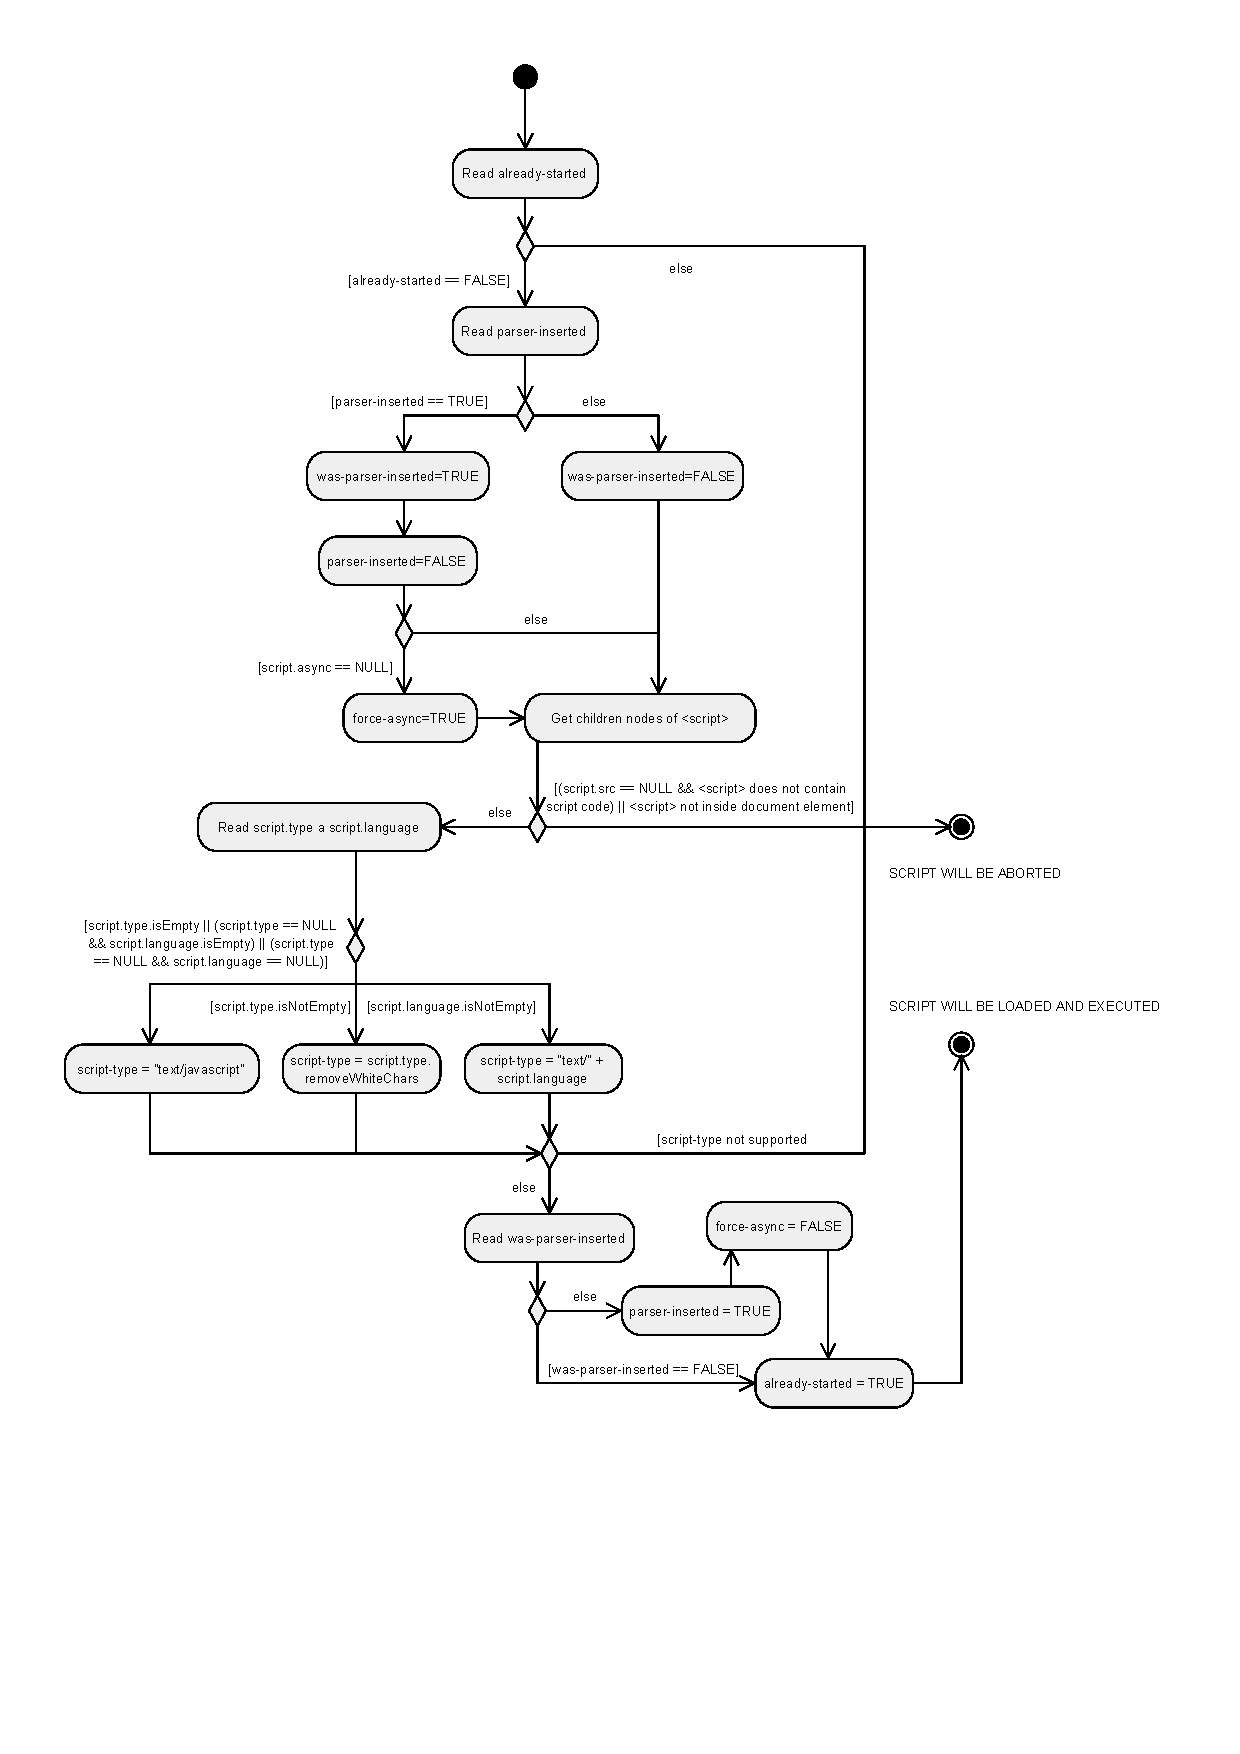
\includegraphics{fig/script-preparation-steps.pdf}
    }
    \caption{Diagram aktivit znázorňující kroky přípravy skriptu před jeho vykonáním}
    \label{Figure.ScriptPreparationSteps}
  \end{center}
\end{figure}

\chapter{Manuál}
\label{Annex.manual}

\chapter{Popis balíků projektu}
\label{Annex.packageDescription}

Následující seznam obsahuje popis nejdůležitějších balíků projektů. Z cest balíků byla vynechána 
cesta k hlavního balíku projektu \texttt{org/fit/cssbox/scriptbox}.

\begin{itemize}
  \item[] \textbf{browser/} -- aaaaaa;
  \item[] \textbf{demo/} -- aaaaaa;
     \begin{itemize}
       \item[] \textbf{browser/} -- aaaaaa;
       \item[] \textbf{tester/} -- aaaaaa;
     \end{itemize}
  \item[] \textbf{dom/} -- aaaaaa;
     \begin{itemize}
       \item[] \textbf{events/} -- aaaaaa;
         \begin{itemize}
           \item[] \textbf{adapters/} -- aaaaaa;
           \item[] \textbf{script/} -- aaaaaa;
         \end{itemize}
       \item[] \textbf{interfaces/} -- aaaaaa;
     \end{itemize}
  \item[] \textbf{events/} -- aaaaaa;
  \item[] \textbf{exceptions/} -- aaaaaa;
  \item[] \textbf{history/} -- aaaaaa;
  \item[] \textbf{misc/} -- aaaaaa;
  \item[] \textbf{navigation/} -- aaaaaa;
  \item[] \textbf{parser/} -- aaaaaa;
  \item[] \textbf{reource/} -- aaaaaa;
     \begin{itemize}
       \item[] \textbf{content/} -- aaaaaa;
         \begin{itemize}
           \item[] \textbf{handlers/} -- aaaaaa;
         \end{itemize}
       \item[] \textbf{fetch/} -- aaaaaa;
         \begin{itemize}
           \item[] \textbf{handlers/} -- aaaaaa;
         \end{itemize}
     \end{itemize}
  \item[] \textbf{script/} -- aaaaaa;
     \begin{itemize}
       \item[] \textbf{adapter/} -- aaaaaa;
       \item[] \textbf{annotation/} -- aaaaaa;
       \item[] \textbf{exceptions/} -- aaaaaa;
       \item[] \textbf{injectors/} -- aaaaaa;
       \item[] \textbf{javascript/} -- aaaaaa;
         \begin{itemize}
           \item[] \textbf{injectors/} -- aaaaaa;
           \item[] \textbf{java/} -- aaaaaa;
           \item[] \textbf{wrap/} -- aaaaaa;
         \end{itemize}
       \item[] \textbf{reflect/} -- aaaaaa;
     \end{itemize}
  \item[] \textbf{security/} -- aaaaaa;
     \begin{itemize}
       \item[] \textbf{origins/} -- aaaaaa;
     \end{itemize}
  \item[] \textbf{ui/} -- aaaaaa;
  \item[] \textbf{url/} -- aaaaaa;
  \item[] \textbf{window/} -- aaaaaa;
\end{itemize}

%\chapter{Konfigrační soubor}
%\chapter{RelaxNG Schéma konfiguračního soboru}
%\chapter{Plakat}

